
%% bare_conf.tex
%% V1.3
%% 2007/01/11
%% by Michael Shell
%% See:
%% http://www.michaelshell.org/
%% for current contact information.\emph{}
%%
%% This is a skeleton file demonstrating the use of IEEEtran.cls
%% (requires IEEEtran.cls version 1.7 or later) with an IEEE conference paper.
%%
%% Support sites:
%% http://www.michaelshell.org/tex/ieeetran/
%% http://www.ctan.org/tex-archive/macros/latex/contrib/IEEEtran/
%% and little change
%% http://www.ieee.org/

%%*************************************************************************
%% Legal Notice:
%% This code is offered as-is without any warranty either expressed or
%% implied; without even the implied warranty of MERCHANTABILITY or
%% FITNESS FOR A PARTICULAR PURPOSE!
%% User assumes all risk.
%% In no event shall IEEE or any contributor to this code be liable for
%% any damages or losses, including, but not limited to, incidental,
%% consequential, or any other damages, resulting from the use or misuse
%% of any information contained here.
%%
%% All comments are the opinions of their respective authors and are not
%% necessarily endorsed by the IEEE.
%%
%% This work is distributed under the LaTeX Project Public License (LPPL)
%% ( http://www.latex-project.org/ ) version 1.3, and may be freely used,
%% distributed and modified. A copy of the LPPL, version 1.3, is included
%% in the base LaTeX documentation of all distributions of LaTeX released
%% 2003/12/01 or later.
%% Retain all contribution notices and credits.
%% ** Modified files should be clearly indicated as such, including  **
%% ** renaming them and changing author support contact information. **
%%
%% File list of work: IEEEtran.cls, IEEEtran_HOWTO.pdf, bare_adv.tex,
%%                    bare_conf.tex, bare_jrnl.tex, bare_jrnl_compsoc.tex
%%*************************************************************************

% *** Authors should verify (and, if needed, correct) their LaTeX system  ***
% *** with the testflow diagnostic prior to trusting their LaTeX platform ***
% *** with production work. IEEE's font choices can trigger bugs that do  ***
% *** not appear when using other class files.                            ***
% The testflow support page is at:
% http://www.michaelshell.org/tex/testflow/



% Note that the a4paper option is mainly intended so that authors in
% countries using A4 can easily print to A4 and see how their papers will
% look in print - the typesetting of the document will not typically be
% affected with changes in paper size (but the bottom and side margins will).
% Use the testflow package mentioned above to verify correct handling of
% both paper sizes by the user's LaTeX system.
%
% Also note that the "draftcls" or "draftclsnofoot", not "draft", option
% should be used if it is desired that the figures are to be displayed in
% draft mode.
%
%\documentclass[conference]{IEEEtran}
\documentclass[conference]{IEEEtran}

% Add the compsoc option for Computer Society conferences.
%
% If IEEEtran.cls has not been installed into the LaTeX system files,
% manually specify the path to it like:
% \documentclass[conference]{../sty/IEEEtran}


\usepackage{graphicx}
\usepackage{algorithm}
%\usepackage{algorithmic}
\usepackage{algpseudocode}
\usepackage[tight,footnotesize]{subfigure}
\usepackage{amsmath}
\usepackage{amsfonts}
\usepackage{amssymb}
\usepackage{url}
\usepackage{cite}

% *** GRAPHICS RELATED PACKAGES ***
%
\usepackage{epsfig}
\usepackage{float}
\usepackage{textcomp}
\usepackage[T1]{fontenc}  % access \textquotedbl
\usepackage{textcomp}     % access \textquotesingle
\graphicspath{{./figures/}}


% Some very useful LaTeX packages include:
% (uncomment the ones you want to load)


% *** MISC UTILITY PACKAGES ***
%
%\usepackage{ifpdf}
% Heiko Oberdiek's ifpdf.sty is very useful if you need conditional
% compilation based on whether the output is pdf or dvi.
% usage:
% \ifpdf
%   % pdf code
% \else
%   % dvi code
% \fi
% The latest version of ifpdf.sty can be obtained from:
% http://www.ctan.org/tex-archive/macros/latex/contrib/oberdiek/
% Also, note that IEEEtran.cls V1.7 and later provides a builtin
% \ifCLASSINFOpdf conditional that works the same way.
% When switching from latex to pdflatex and vice-versa, the compiler may
% have to be run twice to clear warning/error messages.






% *** CITATION PACKAGES ***
%
%\usepackage{cite}
% cite.sty was written by Donald Arseneau
% V1.6 and later of IEEEtran pre-defines the format of the cite.sty package
% \cite{} output to follow that of IEEE. Loading the cite package will
% result in citation numbers being automatically sorted and properly
% "compressed/ranged". e.g., [1], [9], [2], [7], [5], [6] without using
% cite.sty will become [1], [2], [5]--[7], [9] using cite.sty. cite.sty's
% \cite will automatically add leading space, if needed. Use cite.sty's
% noadjust option (cite.sty V3.8 and later) if you want to turn this off.
% cite.sty is already installed on most LaTeX systems. Be sure and use
% version 4.0 (2003-05-27) and later if using hyperref.sty. cite.sty does
% not currently provide for hyperlinked citations.
% The latest version can be obtained at:
% http://www.ctan.org/tex-archive/macros/latex/contrib/cite/
% The documentation is contained in the cite.sty file itself.






% *** GRAPHICS RELATED PACKAGES ***
%
\ifCLASSINFOpdf
  % \usepackage[pdftex]{graphicx}
  % declare the path(s) where your graphic files are
  % \graphicspath{{../pdf/}{../jpeg/}}
  % and their extensions so you won't have to specify these with
  % every instance of \includegraphics
  % \DeclareGraphicsExtensions{.pdf,.jpeg,.png}
\else
  % or other class option (dvipsone, dvipdf, if not using dvips). graphicx
  % will default to the driver specified in the system graphics.cfg if no
  % driver is specified.
  % \usepackage[dvips]{graphicx}
  % declare the path(s) where your graphic files are
  % \graphicspath{{../eps/}}
  % and their extensions so you won't have to specify these with
  % every instance of \includegraphics
  % \DeclareGraphicsExtensions{.eps}
\fi
% graphicx was written by David Carlisle and Sebastian Rahtz. It is
% required if you want graphics, photos, etc. graphicx.sty is already
% installed on most LaTeX systems. The latest version and documentation can
% be obtained at:
% http://www.ctan.org/tex-archive/macros/latex/required/graphics/
% Another good source of documentation is "Using Imported Graphics in
% LaTeX2e" by Keith Reckdahl which can be found as epslatex.ps or
% epslatex.pdf at: http://www.ctan.org/tex-archive/info/
%
% latex, and pdflatex in dvi mode, support graphics in encapsulated
% postscript (.eps) format. pdflatex in pdf mode supports graphics
% in .pdf, .jpeg, .png and .mps (metapost) formats. Users should ensure
% that all non-photo figures use a vector format (.eps, .pdf, .mps) and
% not a bitmapped formats (.jpeg, .png). IEEE frowns on bitmapped formats
% which can result in "jaggedy"/blurry rendering of lines and letters as
% well as large increases in file sizes.
%
% You can find documentation about the pdfTeX application at:
% http://www.tug.org/applications/pdftex





% *** MATH PACKAGES ***
%
%\usepackage[cmex10]{amsmath}
% A popular package from the American Mathematical Society that provides
% many useful and powerful commands for dealing with mathematics. If using
% it, be sure to load this package with the cmex10 option to ensure that
% only type 1 fonts will utilized at all point sizes. Without this option,
% it is possible that some math symbols, particularly those within
% footnotes, will be rendered in bitmap form which will result in a
% document that can not be IEEE Xplore compliant!
%
% Also, note that the amsmath package sets \interdisplaylinepenalty to 10000
% thus preventing page breaks from occurring within multiline equations. Use:
%\interdisplaylinepenalty=2500
% after loading amsmath to restore such page breaks as IEEEtran.cls normally
% does. amsmath.sty is already installed on most LaTeX systems. The latest
% version and documentation can be obtained at:
% http://www.ctan.org/tex-archive/macros/latex/required/amslatex/math/





% *** SPECIALIZED LIST PACKAGES ***
%
%\usepackage{algorithmic}
% algorithmic.sty was written by Peter Williams and Rogerio Brito.
% This package provides an algorithmic environment fo describing algorithms.
% You can use the algorithmic environment in-text or within a figure
% environment to provide for a floating algorithm. Do NOT use the algorithm
% floating environment provided by algorithm.sty (by the same authors) or
% algorithm2e.sty (by Christophe Fiorio) as IEEE does not use dedicated
% algorithm float types and packages that provide these will not provide
% correct IEEE style captions. The latest version and documentation of
% algorithmic.sty can be obtained at:
% http://www.ctan.org/tex-archive/macros/latex/contrib/algorithms/
% There is also a support site at:
% http://algorithms.berlios.de/index.html
% Also of interest may be the (relatively newer and more customizable)
% algorithmicx.sty package by Szasz Janos:
% http://www.ctan.org/tex-archive/macros/latex/contrib/algorithmicx/




% *** ALIGNMENT PACKAGES ***
%
%\usepackage{array}
% Frank Mittelbach's and David Carlisle's array.sty patches and improves
% the standard LaTeX2e array and tabular environments to provide better
% appearance and additional user controls. As the default LaTeX2e table
% generation code is lacking to the point of almost being broken with
% respect to the quality of the end results, all users are strongly
% advised to use an enhanced (at the very least that provided by array.sty)
% set of table tools. array.sty is already installed on most systems. The
% latest version and documentation can be obtained at:
% http://www.ctan.org/tex-archive/macros/latex/required/tools/


%\usepackage{mdwmath}
%\usepackage{mdwtab}
% Also highly recommended is Mark Wooding's extremely powerful MDW tools,
% especially mdwmath.sty and mdwtab.sty which are used to format equations
% and tables, respectively. The MDWtools set is already installed on most
% LaTeX systems. The lastest version and documentation is available at:
% http://www.ctan.org/tex-archive/macros/latex/contrib/mdwtools/


% IEEEtran contains the IEEEeqnarray family of commands that can be used to
% generate multiline equations as well as matrices, tables, etc., of high
% quality.


%\usepackage{eqparbox}
% Also of notable interest is Scott Pakin's eqparbox package for creating
% (automatically sized) equal width boxes - aka "natural width parboxes".
% Available at:
% http://www.ctan.org/tex-archive/macros/latex/contrib/eqparbox/





% *** SUBFIGURE PACKAGES ***
%\usepackage[tight,footnotesize]{subfigure}
% subfigure.sty was written by Steven Douglas Cochran. This package makes it
% easy to put subfigures in your figures. e.g., "Figure 1a and 1b". For IEEE
% work, it is a good idea to load it with the tight package option to reduce
% the amount of white space around the subfigures. subfigure.sty is already
% installed on most LaTeX systems. The latest version and documentation can
% be obtained at:
% http://www.ctan.org/tex-archive/obsolete/macros/latex/contrib/subfigure/
% subfigure.sty has been superceeded by subfig.sty.



%\usepackage[caption=false]{caption}
%\usepackage[font=footnotesize]{subfig}
% subfig.sty, also written by Steven Douglas Cochran, is the modern
% replacement for subfigure.sty. However, subfig.sty requires and
% automatically loads Axel Sommerfeldt's caption.sty which will override
% IEEEtran.cls handling of captions and this will result in nonIEEE style
% figure/table captions. To prevent this problem, be sure and preload
% caption.sty with its "caption=false" package option. This is will preserve
% IEEEtran.cls handing of captions. Version 1.3 (2005/06/28) and later
% (recommended due to many improvements over 1.2) of subfig.sty supports
% the caption=false option directly:
%\usepackage[caption=false,font=footnotesize]{subfig}
%
% The latest version and documentation can be obtained at:
% http://www.ctan.org/tex-archive/macros/latex/contrib/subfig/
% The latest version and documentation of caption.sty can be obtained at:
% http://www.ctan.org/tex-archive/macros/latex/contrib/caption/




% *** FLOAT PACKAGES ***
%
%\usepackage{fixltx2e}
% fixltx2e, the successor to the earlier fix2col.sty, was written by
% Frank Mittelbach and David Carlisle. This package corrects a few problems
% in the LaTeX2e kernel, the most notable of which is that in current
% LaTeX2e releases, the ordering of single and double column floats is not
% guaranteed to be preserved. Thus, an unpatched LaTeX2e can allow a
% single column figure to be placed prior to an earlier double column
% figure. The latest version and documentation can be found at:
% http://www.ctan.org/tex-archive/macros/latex/base/



%\usepackage{stfloats}
% stfloats.sty was written by Sigitas Tolusis. This package gives LaTeX2e
% the ability to do double column floats at the bottom of the page as well
% as the top. (e.g., "\begin{figure*}[!b]" is not normally possible in
% LaTeX2e). It also provides a command:
%\fnbelowfloat
% to enable the placement of footnotes below bottom floats (the standard
% LaTeX2e kernel puts them above bottom floats). This is an invasive package
% which rewrites many portions of the LaTeX2e float routines. It may not work
% with other packages that modify the LaTeX2e float routines. The latest
% version and documentation can be obtained at:
% http://www.ctan.org/tex-archive/macros/latex/contrib/sttools/
% Documentation is contained in the stfloats.sty comments as well as in the
% presfull.pdf file. Do not use the stfloats baselinefloat ability as IEEE
% does not allow \baselineskip to stretch. Authors submitting work to the
% IEEE should note that IEEE rarely uses double column equations and
% that authors should try to avoid such use. Do not be tempted to use the
% cuted.sty or midfloat.sty packages (also by Sigitas Tolusis) as IEEE does
% not format its papers in such ways.





% *** PDF, URL AND HYPERLINK PACKAGES ***
%
%\usepackage{url}
% url.sty was written by Donald Arseneau. It provides better support for
% handling and breaking URLs. url.sty is already installed on most LaTeX
% systems. The latest version can be obtained at:
% http://www.ctan.org/tex-archive/macros/latex/contrib/misc/
% Read the url.sty source comments for usage information. Basically,
% \url{my_url_here}.





% *** Do not adjust lengths that control margins, column widths, etc. ***
% *** Do not use packages that alter fonts (such as pslatex).         ***
% There should be no need to do such things with IEEEtran.cls V1.6 and later.
% (Unless specifically asked to do so by the journal or conference you plan
% to submit to, of course. )


% correct bad hyphenation here
\hyphenation{op-tical net-works semi-conduc-tor}


\begin{document}
%
% paper title
% can use linebreaks \\ within to get better formatting as desired

\title{EMG-based human-machine interface to control multimedia}

\author{\IEEEauthorblockN{Mohamed Tahar Hammi, Zahra Maatou, Osman Salem and Ahmed Mehaoua}
\IEEEauthorblockA{LIPADE Laboratory, University of Paris Descartes, France\\
\{firstname.lastname\}@parisdescartes.fr}\\ }




% author names and affiliations
% use a multiple column layout for up to three different
% affiliations



% conference papers do not typically use \thanks and this command
% is locked out in conference mode. If really needed, such as for
% the acknowledgment of grants, issue a \IEEEoverridecommandlockouts
% after \documentclass

% for over three affiliations, or if they all won't fit within the width
% of the page, use this alternative format:
%
%\author{\IEEEauthorblockN{Michael Shell\IEEEauthorrefmark{1},
%Homer Simpson\IEEEauthorrefmark{2},
%James Kirk\IEEEauthorrefmark{3},
%Montgomery Scott\IEEEauthorrefmark{3} and
%Eldon Tyrell\IEEEauthorrefmark{4}}
%\IEEEauthorblockA{\IEEEauthorrefmark{1}School of Electrical and Computer Engineering\\
%Georgia Institute of Technology,
%Atlanta, Georgia 30332--0250\\ Email: see http://www.michaelshell.org/contact.html}
%\IEEEauthorblockA{\IEEEauthorrefmark{2}Twentieth Century Fox, Springfield, USA\\
%Email: homer@thesimpsons.com}
%\IEEEauthorblockA{\IEEEauthorrefmark{3}Starfleet Academy, San Francisco, California 96678-2391\\
%Telephone: (800) 555--1212, Fax: (888) 555--1212}
%\IEEEauthorblockA{\IEEEauthorrefmark{4}Tyrell Inc., 123 Replicant Street, Los Angeles, California 90210--4321}}




% use for special paper notices
%\IEEEspecialpapernotice{(Invited Paper)}




% make the title area

\maketitle


% IEEEtran.cls defaults to using nonbold math in the Abstract.
% This preserves the distinction between vectors and scalars. However,
% if the conference you are submitting to favors bold math in the abstract,
% then you can use LaTeX's standard command \boldmath at the very start
% of the abstract to achieve this. Many IEEE journals/conferences frown on
% math in the abstract anyway.

% no keywords




% For peer review papers, you can put extra information on the cover
% page as needed:
% \ifCLASSOPTIONpeerreview
% \begin{center} \bfseries EDICS Category: 3-BBND \end{center}
% \fi
%
% For peerreview papers, this IEEEtran command inserts a page break and
% creates the second title. It will be ignored for other modes.
\IEEEpeerreviewmaketitle


% An example of a floating figure using the graphicx package.
% Note that \label must occur AFTER (or within) \caption.
% For figures, \caption should occur after the \includegraphics.
% Note that IEEEtran v1.7 and later has special internal code that
% is designed to preserve the operation of \label within \caption
% even when the captionsoff option is in effect. However, because
% of issues like this, it may be the safest practice to put all your
% \label just after \caption rather than within \caption{}.
%
% Reminder: the "draftcls" or "draftclsnofoot", not "draft", class
% option should be used if it is desired that the figures are to be
% displayed while in draft mode.
%
%\begin{figure}[!t]
%\centering
%\includegraphics[width=2.5in]{myfigure}
% where an .eps filename suffix will be assumed under latex,
% and a .pdf suffix will be assumed for pdflatex; or what has been declared
% via \DeclareGraphicsExtensions.
%\caption{Simulation Results}
%\label{fig_sim}
%\end{figure}

% Note that IEEE typically puts floats only at the top, even when this
% results in a large percentage of a column being occupied by floats.


% An example of a double column floating figure using two subfigures.
% (The subfig.sty package must be loaded for this to work.)
% The subfigure \label commands are set within each subfloat command, the
% \label for the overall figure must come after \caption.
% \hfil must be used as a separator to get equal spacing.
% The subfigure.sty package works much the same way, except \subfigure is
% used instead of \subfloat.
%
%\begin{figure*}[!t]
%\centerline{\subfloat[Case I]\includegraphics[width=2.5in]{subfigcase1}%
%\label{fig_first_case}}
%\hfil
%\subfloat[Case II]{\includegraphics[width=2.5in]{subfigcase2}%
%\label{fig_second_case}}}
%\caption{Simulation results}
%\label{fig_sim}
%\end{figure*}
%
% Note that often IEEE papers with subfigures do not employ subfigure
% captions (using the optional argument to \subfloat), but instead will
% reference/describe all of them (a), (b), etc., within the main caption.


% An example of a floating table. Note that, for IEEE style tables, the
% \caption command should come BEFORE the table. Table text will default to
% \footnotesize as IEEE normally uses this smaller font for tables.
% The \label must come after \caption as always.
%
%\begin{table}[!t]
%% increase table row spacing, adjust to taste
%\renewcommand{\arraystretch}{1.3}
% if using array.sty, it might be a good idea to tweak the value of
% \extrarowheight as needed to properly center the text within the cells
%\caption{An Example of a Table}
%\label{table_example}
%\centering
%% Some packages, such as MDW tools, offer better commands for making tables
%% than the plain LaTeX2e tabular which is used here.
%\begin{tabular}{|c||c|}
%\hline
%One & Two\\
%\hline
%Three & Four\\
%\hline
%\end{tabular}
%\end{table}


%%%%%%%%%%%%%%%%%%%%%%%%%%%%%%%%%%%%%%%%%%%%%%%%%%%%%%%%%%
\begin{abstract}
%%%%%%%%%%%%%%%%%%%%%%%%%%%%%%%%%%%%%%%%%%%%%%%%%%%%%%%%%%
The EMG signals acquired from muscles are used in high-tech fields such as augmented reality,
biomedical, gaming, 3D animations, human-machine interfaces.
These human-machine interfaces are used especialy for helping people with reduced mobility or that have special needs to control machines.
The purpose of this paper is to realise a novel, flexible and efficient system EMG-based, to control a multimedia, 
using a microcontroller and a programming language. First numerous  evaluations were done to validate our apporoach.
Thene these evaluations . A
comparison study is also given to show performance of va
rious EMG signal analysis methods. This paper provides
researchers a good understanding of EMG signal and its anal
ysis procedures. This knowledge will help them develop
more s. 


In order to validate our proposal, firstly, .\par

\end{abstract}
%%%%%%%%%%%%%%%%%%%%%%%%%%%%%%%%%%%%%%%%%%%%%%%%%%%%%%%%%%
\begin{keywords}
EMG, muscle, signal processing, media player, control interface
\end{keywords}
%%%%%%%%%%%%%%%%%%%%%%%%%%%%%%%%%%%%%%%%%%%%%%%%%%%%%%%%%%
%%%%%%%%%%%%%%%%%%%%%%%%%%%%%%%%%%%%%%%%%%%%%%%%%%%%%%%%%%%%%%%%%%%%%%%%%
\section{Introduction}
%%%%%%%%%%%%%%%%%%%%%%%%%%%%%%%%%%%%%%ffffff%%%%%%%%%%%%%%%%%%%%%%%%%%%%%%%%%%%

The discovery of the Electromyogram (EMG) signal was in 1666, when the Italian "Francesco Redi" has shown that the muscle can generate an electric current. After two centuries,  in 1849, the German-French researcher "Dubois-Reymond" was the first whom realized the first record of an EMG signal.

The EMG signal is generated as a result of a depolarization followed by a repolarization that happen at the entrance of the sodium in the interior of the cell membrane of a skeletal muscle fiber, and release potassium to the outside. ~\cite{Konte}. \par

%%%%%%%%%%%%%%%%%%%%%%%%%%%%%%%%%%%%%%%%%%%%%%%%%%%%%%%%%%%%%%%%%%%%%%%%%%%%%%
Nowadays, the EMG signal provides an intelligent and natural way of a human machine interaction, which can be a good solution to replace conventional controls interfaces and allows some categories of users the opportunity to exploit the new technologies. Amputation and deformity have been dealt with, one way or
another, throughout the ages. More than one million individuals in the United States today are living with limb amputations ~\cite{Patricia}, in which there are approximately
100,000 patients with an upper limb amputation. According to~\cite{China} approximately 8\% of physical disables, or 2.26 million people,
live with limb amputations in China alone. Natural disasters and accidents have been making this number increase.
\par
The use of EMG is not limited to the field of medicine, but it is also convenient for the other technology fields, which is explained by the diversity of the applications that we can be found today.
\par
%Electromyography (EMG) is a technique for evaluating and recording the electrical activity, is realized by using an instrument called an electromyograph, to produce a record called an electromyogram. \par
%%%%%%%%%%%%%%%%%%%%%%%%%%%%%%%%%%fffff%%%%%%%%%%%%%%%%%%%%%%%%%%%%%%%%%%%%%%%
Several researches and applications have treated the EMG signals. In fact, numerous studies have been made on classifications and treatments of it. for instance, on facial expressions recognition by analyzing physiological signals, on detection and identification of the uterine EMG signal for prediction of premature child-birth.
Our study is focused on the EMG signals generated by a human hand or arm.  We aim to develop an application that controls a set of media, using the EMG signal with arm force. The electrical potential generated during a contraction of an arm muscles permits to start a video or switch between a set of media. Our proposed system has been developed in the purpose of creating an EMG-based remote control that allows more simplicity to use than the classical methods, especially for helping people with reduced mobility.


The rest of this paper is organized as follows.
Section~\ref{sec:related} reviews relevant related work and different existing approaches for exploiting the EMG signals. Section~\ref{sec:proposedapproach} presents our approach for using the EMG signals to take control over a multimedia application that we have implemented in C++, and we present some tests that we have done and their results . Section~\ref{sec:conclusion} concludes this paper and presents some perspectives for our futur work.\par
%%%%%%%%%%%%%%%%%%%%%%%%%%%%%%%%%%%%%%%%%%%%%%%%%%%%%%%%%%%%%%%%%%%%%%%%%%%%%%%%%%%%%%%%%%%%%%%%%%%%%%%%%%%%%%%%%%%%%%%%%%%%%%%%%%%%%%%%%%%%%%%%%%
\section{Related work} \label{sec:related}


Numerous studies have been made in the area of EMG. ~\cite{Hamdi} showed that the EMG allows to measure the facial electrical activity of muscles via electrodes placed on the face, this measure can be used for expressions recognition. From this facial expressions we can distinguish a stress which causes an increase muscular activity and many others expressions as negative valence, lack of motivation ...ect. \par

Its approach consists to realise an immersive simulation platform for job interviews, which is based on a set of sensors which are used to acquire physiological signals (EMG, ECG ...). These signals are processed as follows (extraction, characteristics, classification and performance evaluation of classifiers). The purpose of this platform is to improve the candidate's behavioral skills and training him to manage his emotional state by using the data that is gathered from him.\par

The system can give a misinterpretation of the user's face, but in general it remains a good work that brings a new solution that did not exist before, which can be very handy if some improvements were added.\par
%%%%%%%%%%%%%%%%%%%%%%%%%%%%%%%%%%%%%%%%%%%%%%%%%%%%%%%%%%%%%%%%%%%%%%%%%%%%%%%%%%%%%%%%%%%%%%%%%%%%%%%%%%%%%%%%%%%%%%%%%%%%%%%%%%%%%%%%%%%%%%%%%%
%%%%%%%%%%%%%%%%%%%%%%%%%%%%%%%%%%%%%%%%%%%%%%%%%%%%%%%%%%%%%%%%%%%%%%%%%
The EMG signal can enable better monitoring of the contraction's evolution during the pregnancy~\cite{Chendab} .\par Indeed, the precocious detection of premature child-birth is the key of prevention. The treatment method of EMG uterine for detecting and identifying the pertinent events is based on the wavelet packets.
The author propose two approaches for an EMG uterine decomposition, discrete wavelet decomposition which consists to decompose the EMG signal according to the scale levels. this scale interprets any change in frequency or energy signal. And the second approach is the wavelet packet decomposition which is based on the construction of sub-basic functions organized into packets.
These approachs permit to choose the most pertinent packages for the good detection and classification of an EMG uterine. Furthermore, we can use other types of frequency wavelet that are more selective.\par
%%%%%%%%%%%%%%%%%%%%%%%%%%%%%%%%%%%%%%%%%%%%%%%%%%%%%%%%%%%%%%%%%%%%%%%%%%
Several methods in ~\cite{huet} are successively applied on the EMG signals so it can be interpreted. The important step is to extract the most discriminative features. Then, various types of classifiers may be used, each one of them presents advantages and disadvantages. None of them for the moment won unanimously. The objective of these classifiers is to choose a reliable and fast learning mechanism, a way to be adapted to control a hand prosthesis.\par

These classifiers are poorly adapted to the changes of the signals occurring from different operators over the time.\par
%%%%%%%%%%%%%%%%%%%%%%%%%%%%%%%%%%%%%%%%%%%%%%%%%%%%%%%%%%%%%%%%%%%%%%%%%


%%%%%%%%%%%%%%%%%%%%%%%%%%%%%%%%%%%%%%%%%%%%%%%%%%%%%%%%%%%%%%%%%%%%%%%%%
Author in ~\cite{LeCarpentier} treat the problem of EMG signal decomposition based on the observation from a single sensor. According to it and to ~\cite{DeLuca}, the decomposition consists in the restitution of pulse train for each motor unit corresponding, and enables the subsequent analysis of muscle motor units proprieties, providing an interpretation of the neural roles in the muscle. The decomposition process is performed in two steps: pretreatment for segmenting the EMG signal and provide an approximation of the shapes of elementary waves, followed by a "Bayesian decomposition" that use the stochastic simulation approach, (MCMC).
The strength of this solution is that, unlike existing methods, no human manipulation is involved in this process, both steps are fully automatic. This work is bringing a new solution, however it lacks a technical implementation in addition to simulation that has been achieved.\par%%%%%%%%%%%%%%%%%%%%%%%%%%%%%%%%%%%%%%%%%%%%%%%%%%%%%%%%%%%%%%%%%%%%%%%%%
Authors in ~\cite{Artemiadis} propose a new method that allow users to control an anthropomorphic robot arm in a 3D space, by developing an interface between the user and the robot arm which is controlled by EMG signals. The efficacy of this proposition is that the experiments are done in real time, including random arm motions with variable hand speed profiles, and those arm motions are not affected by EMG changes with respect to time, and that is done by using a switching model in such a way that it compensated for the EMG changes. This solution is very convenient but the only problem is that the use of robots is not within the reach of everyone and it can be very expensive.\par
%%%%%%%%%%%%%%%%%%%%%%%%%%%%%%%%%%%%%%%%%%%%%%%%%%%%%%%%%%%%%%%%%%%%%%%%%
Studies in~\cite{Zhang} describes a new hand gesture recognition system based on both multi-channel surface EMG sensors and 3D ACC (accelerometer) to realize a flexible interaction between human and computers. The set of defined hand gestures include both finger actions and circular hand movements of various orientations. To evaluate their system they implemented an application that allow to control Virtual Rubik's Cube game. This work is very interesting because it combines two sensing techniques for hand gestures recognition, thus, precision and efficiency are enhanced. However, this application is not that practical for people whom cannot move their hands in a proper way (circular movements of various orientations).\par
%%%%%%%%%%%%%%%%%%%%%%%%%%%%%%%%%%%%%%%%%%%%%%%%%%%%%%%%%%%%%%%%%%%%%%%%%
Authors in~\cite{Atieh} propose an interface of "control command" between the prosthetic hand and the human. The human communicates with the prosthetic by sending commands "to keep a hand open, to keep pincer position, keep a encompassing entry position,..etc. On the other hand, the prosthetic hand communicates with the human by displaying messages that are:\par
Send error messages (when the system does not know the signal value). Raise an alarm in case of fatigue. View the status of the battery.\par
This solution allows creation of a simple and useful prosthetic hand which is easy to use. But the main problems that we can encounter, is when error messages are displayed on the screen in the case of a co-contraction (contraction of two muscles in the same time), when the prosthetic receives an unknown signal, and when the amplitude of the signal does not indicate a weak nor a strong contraction (between the two).\par
In addition this solution is not optimal nor flexible because when we want to move from an encompassing state to a pinching state , we have to go through an open state.\par
Finally, this work has not been implemented yet, so we cannot know what technical problems that can be encountered. \par

%%%%%%%%%%%%%%%%%%%%%%%%%%%%%%%%%%%%%%%%%%%%%%%%%%%%%%%%%%%%%%%%%%%%%%%%

%%%%%%%%%%%%%%%%%%%%%%%%%%%%%%%%%%%%%%%%%%%%%%%%%%%%%%%%%%%%%%%%%%%%%%%%%
In this paper, we aim to develop an application that control set of medias by using EMG signal with hand force. The electrical potential generated during a contraction of muscles arm permit to switch between this set of medias. Our proposed system has developed in the purpose of helping person with reduced mobility. \par
%%%%%%%%%%%%%%%%%%%%%%%%%%%%%%%%%%%%%%%%%%%%%%%%%%%%%%%%%%%%%%%%%%%%%%%%%
%%%%%%%%%%%%%%%%%%%%%%%%%%%%%%%%%%%%%%%%%%%%%%%%%%%%%%%%%%%%%%%%%%%%%%%%%
%%%%%%%%%%%%%%%%%%%%%%%%%%%%%%%%%%%%%%%%%%%%%%%%%%%%%%%%%%%%%%%%%%%%%%%%%
\section{Proposed Approach} \label{sec:proposedapproach}
%%%%%%%%%%%%%%%%%%%%%%%%%%%%%%%%%%%%%%%%%%%%%%%%%%%%%%%%%%%%%%%%%%%%%%%%%
%%%%%%%%%%%%%%%%%%%%%%%%%%%%%%%%%%%%%%%%%%%%%%%%%%%%%%%%%%%%%%%%%%%%%%%%%
%%%%%%%%%%%%%%%%%%%%%%%%%%%%%%%%%%%%%%%%%%%%%%%%%%%%%%%%%%%%%%%%%%%%%%%%%
The control strategies of the application use three electrodes placed on the skin surface overlying the
muscles of the arm in order to gather the EMG signals. In this section we will explain the signal processing in details :


%%%%%%%%%%%%%%%%%%%%%%%%%%%%%%%%%%%%%%%%%%%%%%%%%%%%%%%%%%%%%%%%%%%%%%%%%
\subsection{Electromyography Signal Treatment} \label{sub:EMGsignaltreatment}\par
%%%%%%%%%%%%%%%%%%%%%%%%%%%%%%%%%%%%%%%%%%%%%%%%%%%%%%%%%%%%%%%%%%%%%%%%%
Herein, we present the analysis of the EMG data that we have achieved on the data collected from the arm muscle by three surface electrodes placed on the skin.\par
The EMG signals acquired from muscles require advanced methods for processing which are as follows (loading, rectification, filter, linear envelope and fourier transform) showed in figure~\ref{fig:struct}. The purpose of this treatment is to turn the signals into a usable form  for registration or correlation purposes.\par

\begin{figure}[!hb]
    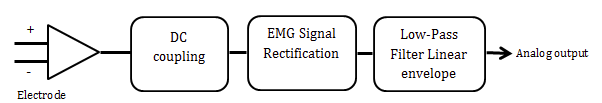
\includegraphics[scale=0.45]{fig0.png}
    \caption{EMG signal processing diagram}
    \label{fig:struct}
\end{figure}


%%%%%%%%%%%%%%%%%%%%%%%%%%%%%%%%%%%%%%%%%%%%%%%%%%%%%%%%%%%%%%%%%%%%%%%%
\subsubsection{Loading the EMG data} \label{sub:LoadingtheEMGdata}\par
This step is a presentation of the data without processing, except an amplification of the signal that can be added by the electrode. The raw signal is presented in figure~\ref{fig:data} .\par

\begin{figure}[!hb]
    \hspace*{1.2 cm}
    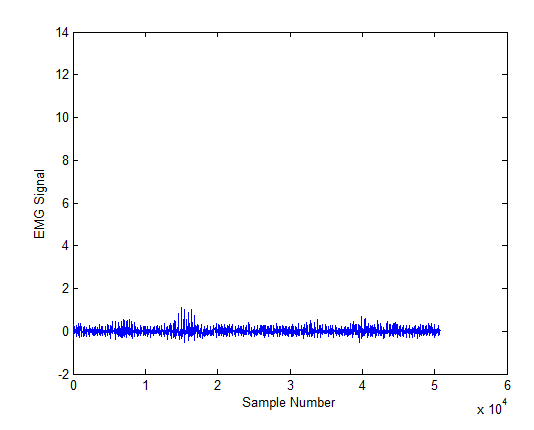
\includegraphics[scale=0.40]{fig1.png}
    \caption{EMG Data}
    \label{fig:data}
\end{figure}

%%%%%%%%%%%%%%%%%%%%%%%%%%%%%%%%%%%%%%%%%%%%%%%%%%%%%%%%%%%%%%%%%%%%%%%%
\subsubsection{Rectification the EMG signal} \label{sub:RectificationtheEMGsignal}\par
A full rectification generates the absolute value of the EMG signals, it can be also called an average value. Two phases can be distinguished to obtain the average value, as follows: eliminating the offset signal by removing the dc-offset and calculating the absolute value. the results are showed in figure~\ref{fig:rect}.\par

\begin{figure}
    \hspace*{1.2 cm}
    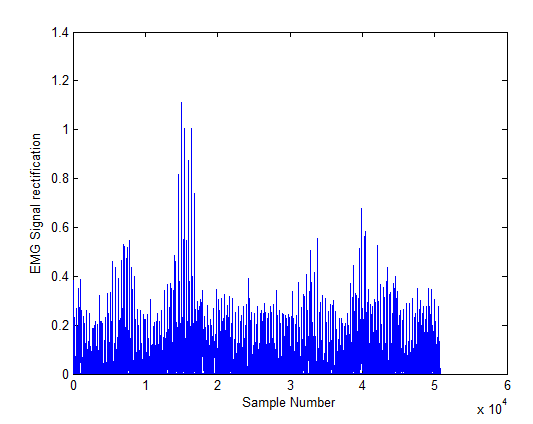
\includegraphics[scale=0.40]{fig2.png}
    \caption{the EMG signal Rectification}
    \label{fig:rect}
\end{figure}

%%%%%%%%%%%%%%%%%%%%%%%%%%%%%%%%%%%%%%%%%%%%%%%%%%%%%%%%%%%%%%%%%%%%%%%%
\subsubsection{Filter and Linear envelope of the EMG signal } \label{sub:LinearenvelopeoftheEMGsignal}\par
Filtering the signal serves to eliminate the unwanted noise, There are three types of noise in a the EMG signal, \par
Bio-electrical noise: that is produced by biological functions, heartbeat, breathing and it can be minimized with good electrodes placement.\par

Equipment noise: it is a noise due to the wires movement, electrodes, skin and amplifiers. the wires noise have a low frequency (10-20 Hz), so filtering at 20 Hz eliminates them. The amplifier's noise is of higher frequencies and it can be found in the upper part of the frequency spectrum of the EMG signal.\par

External noise: All electrical and electromagnetic interference, it can be minimized with a good grounding (GND)

Filters reduce the amplitude of the signal at a given frequency (cutoff frequency), we have used a low pass filter for our treatment of the EMG signal. The cutoff low-pass frequency is often set at around 250 Hz for surface electrode. The linear envelope is the result of a full rectification and low-pass filtering at sampling frequency 2000 Hz, as we can see in figure~\ref{fig:env}.\par

\begin{figure}
    \hspace*{1.2 cm}
    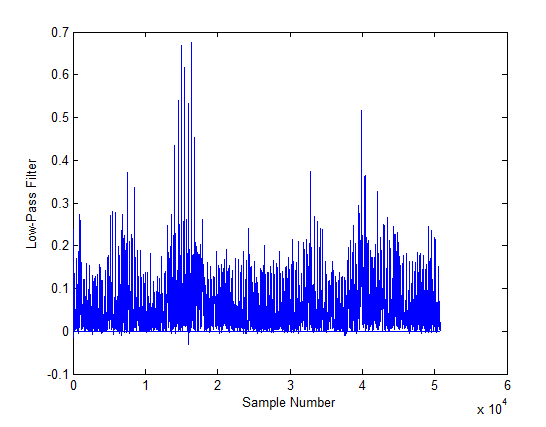
\includegraphics[scale=0.40]{fig3.png}
    \caption{Linear envelope}
    \label{fig:env}
\end{figure}

%%%%%%%%%%%%%%%%%%%%%%%%%%%%%%%%%%%%%%%%%%%%%%%%%%%%%%%%%%%%%%%%%%%%%%%%
\subsubsection{Fourier Transform (FFT) of the EMG signals} \label{sub:FourierTransform(FFT)oftheEMGsignals}
\par The Total Power Spectrum can be calculated by two frequency parameters: Mean Frequency of the FFT as the mathematical mean of the spectrum curve, Total Power as a the integral under the spectrum curve and Median Frequency of the FFT as the parameter that divides the Total Power area into two equal parts~\cite{Konrad} presented in figure~\ref{fig:spectre}. \par
Finally the maximum value of the Total Power Spectrum curve can be used to describe frequency characteristics. Within applied EMG-frequency analysis the most important parameters are the mean and the median frequency and their time domain changes in sustained contractions, which is often employed for analysing muscle fatigue.\par

\begin{figure}
    \hspace*{1.2 cm}
    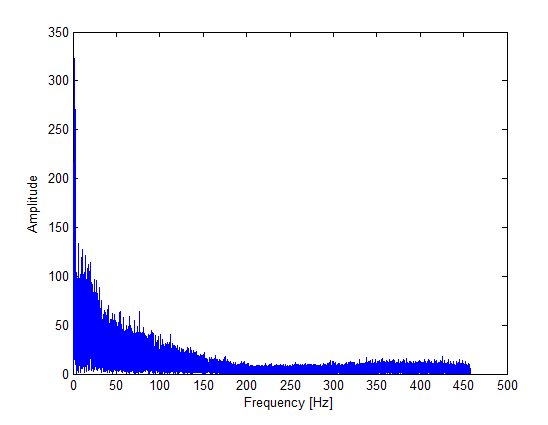
\includegraphics[scale=0.40]{fig4.png}
    \caption{Power Spectrum}
    \label{fig:spectre}
\end{figure}


%%%%%%%%%%%%%%%%%%%%%%%%%%%%%%%%%%%%%%%%%%%%%%%%%%%%%%%%%%%%%%%%%%%%%%%%%%%%%%%%%%%%%%%%%%%%%%%%%%%%%%%%%%%%
%%%%%%%%%%%%%%%%%%%%%%%%%%%%%%%%%%%%%%%%%%%%%%%%%%%%%%%%%%%%%%%%%%%%%%%%%%%%%%%%%%%%%%%%%%%%%%%%%%%%%%%%%%%%
\subsection{Implementation}\par

Figure~\ref{fig:architecture} shows the architecture of our system:

\begin{figure}[!hb]
    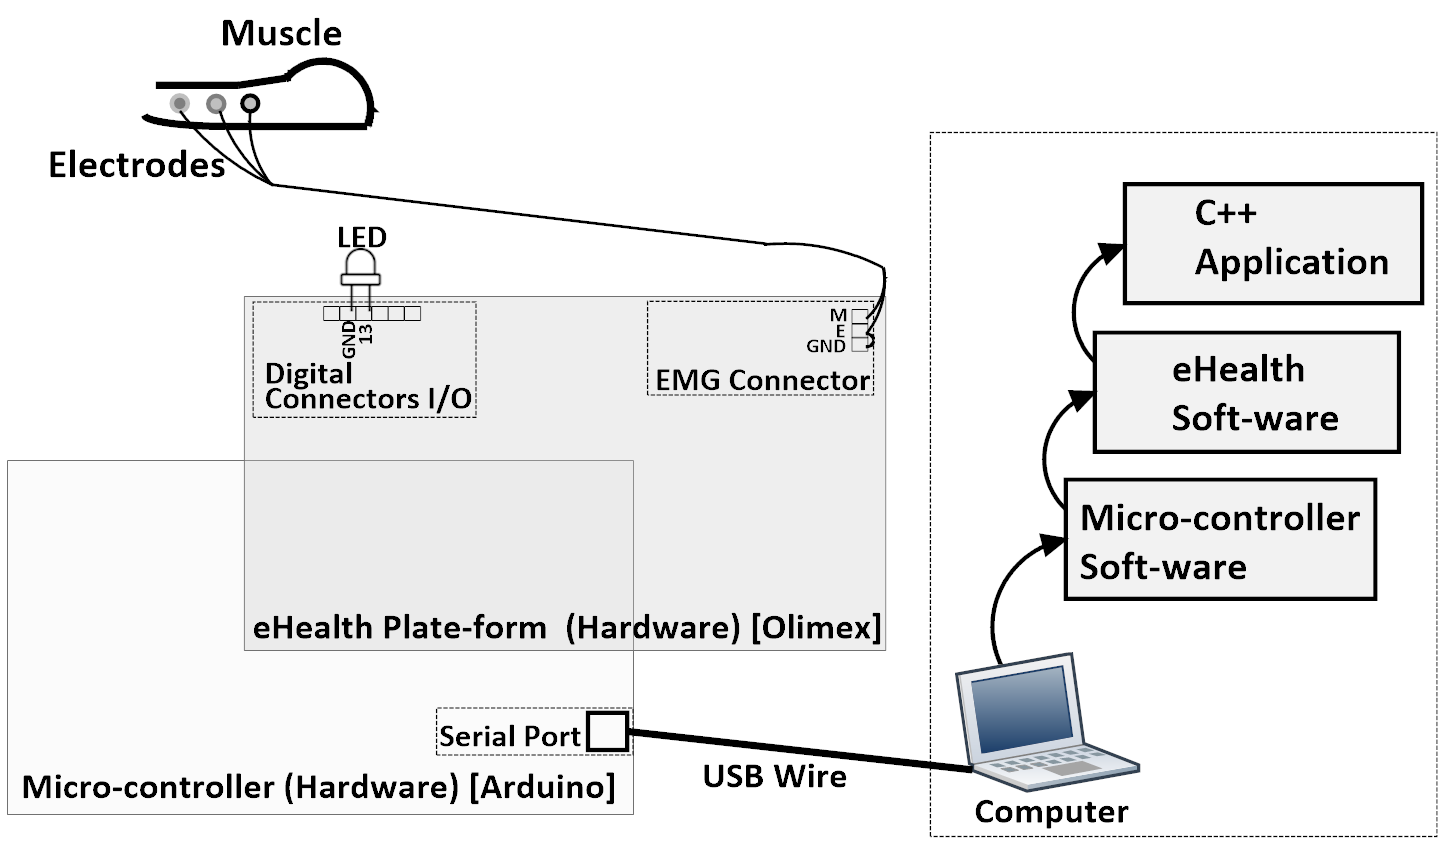
\includegraphics[scale=0.23]{architecture.png}
    \caption{System architecture}
    \label{fig:architecture}
\end{figure}


As seen, the EMG signal is recovered and amplified from muscles via electrodes (3 channels: GND, E and M). Then processed and filtered (as explained above) by the eHealth platform (OLIMEX) attached to a micro-controller (Arduino), this equipement is used to interpret the signal as two values ("ON" and "OFF"), during a contraction a LED turns "ON", and "OFF" in case of rest, this allows the visibility of system operations for the user. The micro-controller can also transfer the filtered signal to our application (C++). This applications gets the signal using a module which is specific for recieving the data from the Serial Port.\par
As mentionned before, the application is written in Qt C++. Qt is a full development framework with tools designed to streamline the creation of applications and user interfaces for desktop, embedded, and mobile platforms ~\cite{Doc}. In our application, we have used 3 modules: QtGui for building the graphical interface, QtCore module which contains core non-GUI functionalities and finaly, Qt phonon module for multimedia applications.
\par
The filtered signal was recovered in a binary form and then, was taken as input data. We started by using its strength as a parameter, so we have devided our signal into two intervals ]l,m] and ]m,n[, which can be interpreted as two commands, the first one is to start the media, and the second one, to switch from one track to another. Figure~\ref{fig:example} show an exemple of use of the application.

\begin{figure}[!hb]
    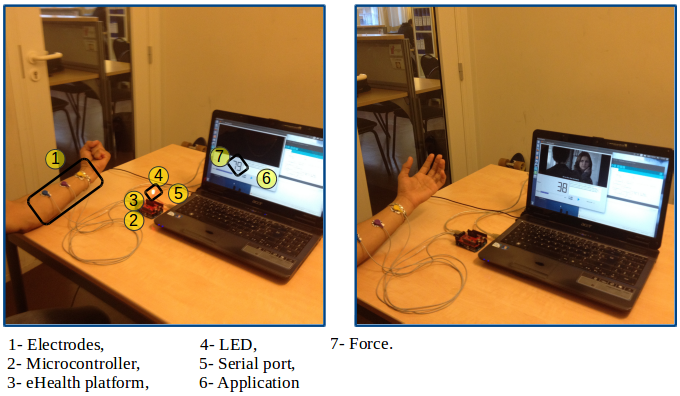
\includegraphics[scale=0.30]{app2.png}
    \caption{Example of use case}
    \label{fig:example}
\end{figure}

So here the user launches the first command to start the first media, we can see also the different components of the interface : a progress bar and an LCDNumber for displaying the signal strength of the user, a button to choose a list of media, and the media viewer. In other words, the user selects a list of media and then controls the mediaplayer with his EMG signal.
\par
To better understand the application's architecture, the following class diagram (Figure~\ref{fig:diagram}) models the multimedia application structure. The "main" class is associated with the "QApplication" and the "control" class which inherits from the "QObject" and is associated with the "QSerialPort" and the "Thread" classes. The "Thread" class inherits from the "QWidget" class and is associated with the "QThread" and the "scene" classes. Finaly, the "scene" class inherits from the "Ui::scene" and the "QMainWindow" classes (this is what we call a multiple inheritance in C++) and is associated with the "phonon" and the "multimedia" classes .

\begin{figure}[!hb]
    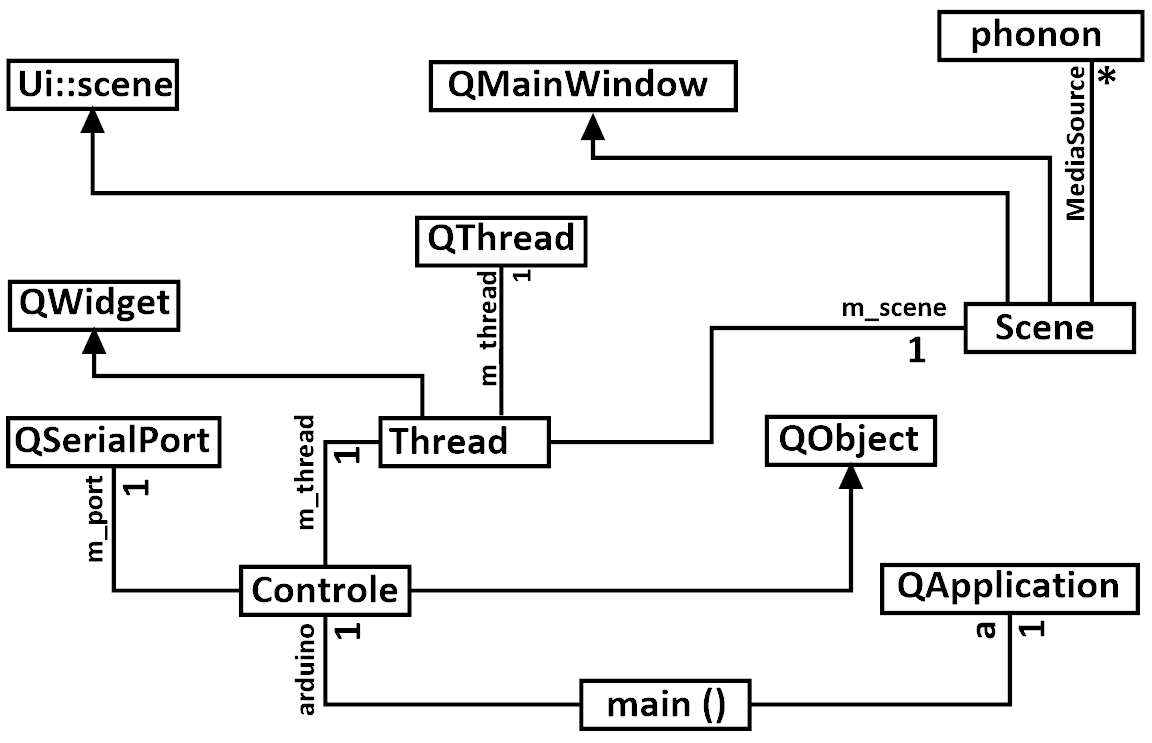
\includegraphics[scale=0.30]{app3.png}
    \caption{class diagram of the C++ application}
    \label{fig:diagram}
\end{figure}

After we tried enhancing and adding new functionalities and, in the same time, keeping the user-friendly side of the system.\par
First, we have done studies on some existing methods allowing an intuitive detection of the location of electrodes and their adaptation with the arm of the user. This step is very important, because The shape and the amplitude of the EMG signal are influenced by the location of the electrodes. Therefore the amplitude of the recorded signal decreases exponentially with respect to the distance between the electrodes and the source of electrical activity. This requires setting up a correction method to simplify the eletrodes placement.\par
Men, Women and children do not have the same EMG signals strength, which requires a learning phase that permits the adaptation of the strength threshold with the proper user. so the approach is that the user -before using the application- has to have some tests done in order to know to which cluster he belongs and that can be done by using a classifiction algorithm (ie : k-means). And, once the category of the user is determined, the system adapts the threshold according to the user.\par

Then, several functionnalities can be added, hence, creating other commands according to three parameters : "Force", "Timing" and "Contraction frequency". So in our application we need to create four commands, C1 : to start the first media or to get the following ones, C2 : to return to the previous media, C3: to pause the media or to continue, C4 : to stop the media.

\begin{table}[h]
    \hspace*{0 cm}
    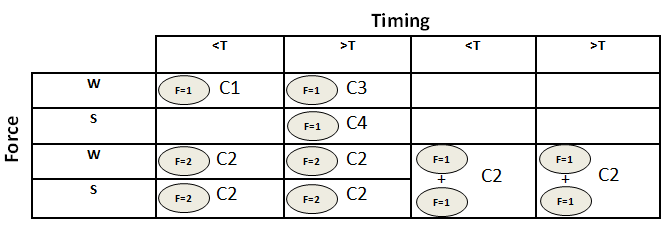
\includegraphics[scale=0.50]{Tableau.png}
    \caption{Commands classification}
    \label{tab:classification}
\end{table}

Table~\ref{tab:classification} shows the combination of different parameters allowing the creation of new commands. When the Force can take two values "Strong" and "Weak", the Timing can take two intervales "<T" and ">T" where T is the time (in seconds) of maintaining the contraction, and F=1, F=2 are respectively Frequency = 1 and Frequency = 2, it's important to know that we must define a maximum time "t" between two frequencies to make the difference between "one command with two frequencies" and between "two different commands". With this combination we can find four commands without any ambiguity. So we can interpret the table as follows : C1(Start|Next) =  W + <T, C2(Previous
) = (2W|2S|S+W)+(<T|T>) which "|" means "or", C3(Pause|Continue) = W + >T, Finally C4(Stop) = S + >T.\par
Then, for a more simplicity, especially for people who cannot move their fingers, we can use a dynamic media list, by creating a file or a database containing links (URLs) downloaded and updated automatically from the Internet.\par
Finally, we made our tests by using wired electrodes that will be replaced later by wireless electrodes, which gives more flexibility, light weight and robustness to our system.\par

\section{Conclusion and futur works} \label{sec:conclusion}
%%%%%%%%%%%%%%%%%%%%%%%%%%%%%%%%%%%%%%%%%%%%%%%%%%%%%%%%%%%%%%%%%%%%%%%%%%%%%%%%
In this paper, we proposed an approach to control a media player by using the EMG signals. Before exploiting the EMG signals, it has to go through some specific processing steps in order to have better results. The approach is designed to provide a control interface destined especially for people with reduced mobility. We have done a real implementation of the application using the OLIMEX eHeath platform, arduino and Qt C++ languages.
To create commands, we have combinated different parameters in order to get a performed interface without any ambiguity on controling it. Our experimental results show that this proposed approach realises an intuitive and user-friendly human machine interface, and it is able to achieve a good performance.
Our future work will focus on the adaptation of this remote on handling multiple applications at once, such as controlling a TV, turn ON and OFF the light of the room, start the robotic vacuum cleaner..etc, while, at the same time,  keeping the flexibility of the system.

%%%%%%%%%%%%%%%%%%%%%%%%%%%%%%%%%%%%%%%%%%%%%%%%%%%%%%%%%%%%%%%%%%%%%%%%%%%%%%%%




% conference papers do not normally have an appendix


% use section* for acknowledgement
%\section*{Acknowledgment}







% trigger a \newpage just before the given reference
% number - used to balance the columns on the last page
% adjust value as needed - may need to be readjusted if
% the document is modified later
%\IEEEtriggeratref{8}
% The "triggered" command can be changed if desired:
%\IEEEtriggercmd{\enlargethispage{-5in}}

% references section

% can use a bibliography generated by BibTeX as a .bbl file
% BibTeX documentation can be easily obtained at:
% http://www.ctan.org/tex-archive/biblio/bibtex/contrib/doc/
% The IEEEtran BibTeX style support page is at:
% http://www.michaelshell.org/tex/ieeetran/bibtex/
\bibliographystyle{IEEEtran}
% argument is your BibTeX string definitions and bibliography database(s)
\bibliography{Securcom}
%
% <OR> manually copy in the resultant .bbl file
% set second argument of \begin to the number of references
% (used to reserve space for the reference number labels box)



% that's all folks
\end{document}

